\documentclass[border=10pt]{standalone}

\usepackage[utf8]{inputenc}                                 % Codificação do documento
\usepackage[T1]{fontenc}                                    % Seleção de código de fonte
\usepackage{microtype}                                      % Melhora a justificação do documento
\usepackage{lmodern}                                        % Usa a fonte Latin Modern
\usepackage{ae, aecompl}                                    % Fontes de alta qualidade

\usepackage{amsmath}
\usepackage{verbatim}
\usepackage{tikz}
\usetikzlibrary{arrows,calc,positioning,shadows.blur,decorations.pathreplacing}
\usepackage{etoolbox}

\usepackage{fontawesome}

\begin{document}
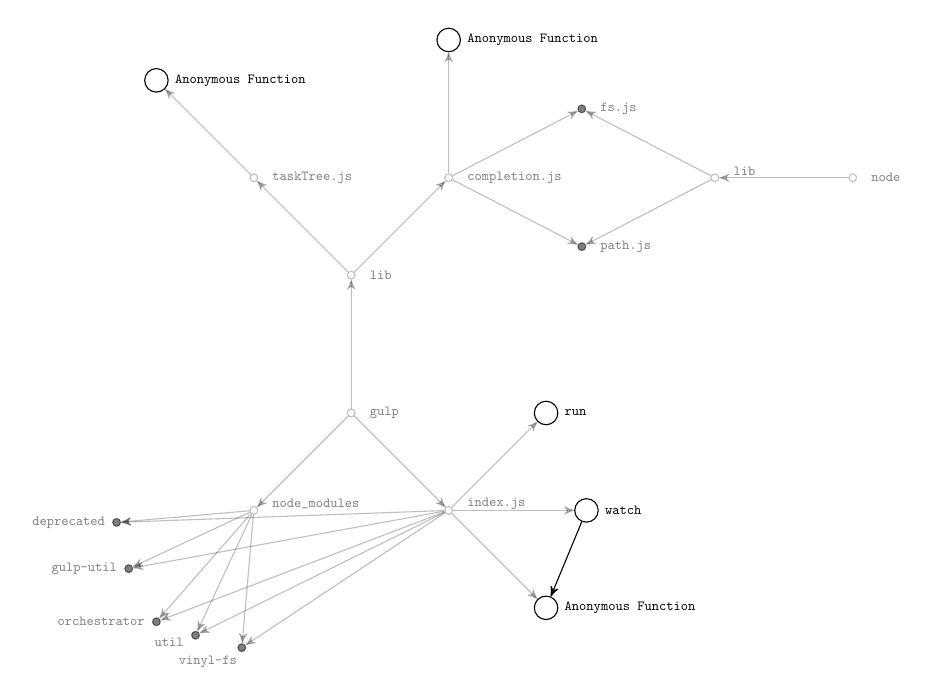
\begin{tikzpicture}
[
                     x =  1.75cm,
	                 y = -1.75cm,
	                ->, >= stealth',
	       node distance = 2cm,
               tv/.style = { draw=black, circle, inner sep=1pt, opacity=0.25 },
	           nv/.style = { draw=black, circle, inner sep=3pt },
			   mv/.style = { draw=black, fill=black, circle, inner sep=1pt, opacity=0.5 },
              dot/.style = { draw=black, fill=black, circle, inner sep=0.75pt },
       coordinate/.style = { draw=none, fill=none, circle, inner sep=0pt, outer sep=0pt },
	   		labe2/.style = { draw=none, fill=none, anchor=east, scale=0.5 },
	        label/.style = { draw=none, fill=none, anchor=west, scale=0.5 },
	     toplabel/.style = { draw=none, fill=none, anchor=north, scale=0.5 }
]

	\node  (1) at (1.414, 2.414) [tv] {};	\node[opacity=0.5]	 (1l) at (1.514, 2.414) [label] {\texttt{gulp}};
	\node  (2) at (0.707, 3.121) [tv] {};	\node[opacity=0.5]	 (2l) at (0.807, 3.071) [label] {\texttt{node\_modules}};
	\node  (3) at (-0.289, 3.208) [mv] {};	\node[opacity=0.5]	 (3l) at (-0.339, 3.208) [labe2] {\texttt{deprecated}};
	\node  (4) at (-0.201, 3.544) [mv] {};	\node[opacity=0.5]	 (4l) at (-0.251, 3.544) [labe2] {\texttt{gulp-util}};
	\node  (5) at (0    , 3.929) [mv] {};	\node[opacity=0.5]	 (5l) at (-0.05 , 3.929) [labe2] {\texttt{orchestrator}};
	\node  (6) at (0.284, 4.027) [mv] {};	\node[opacity=0.5]	 (6l) at (0.234, 4.077) [labe2] {\texttt{util}};
	\node  (7) at (0.62 , 4.117) [mv] {};	\node[opacity=0.5]	 (7l) at (0.62 , 4.217) [labe2] {\texttt{vinyl-fs}};
	\node  (8) at (1.414, 1.414) [tv] {};	\node[opacity=0.5]	 (8l) at (1.514, 1.414) [label] {\texttt{lib}};
	\node  (9) at (2.121, 0.707) [tv] {};	\node[opacity=0.5]	 (9l) at (2.221, 0.707) [label] {\texttt{completion.js}};
	\node (10) at (2.121,-0.293) [nv] {};	\node				(10l) at (2.221,-0.293) [label] {\texttt{Anonymous Function}};
	\node (11) at (0.707, 0.707) [tv] {};	\node[opacity=0.5]	(11l) at (0.807, 0.707) [label] {\texttt{taskTree.js}};
	\node (12) at (0    , 0    ) [nv] {};	\node				(12l) at (0.1  , 0    ) [label] {\texttt{Anonymous Function}};
	\node (13) at (2.121, 3.121) [tv] {};	\node[opacity=0.5]	(13l) at (2.221, 3.071) [label] {\texttt{index.js}};
	\node (14) at (2.828, 2.414) [nv] {};	\node				(14l) at (2.928, 2.414) [label] {\texttt{run}};
	\node (15) at (3.121, 3.121) [nv] {};	\node				(15l) at (3.221, 3.121) [label] {\texttt{watch}};
	\node (16) at (2.828, 3.828) [nv] {};	\node				(16l) at (2.928, 3.828) [label] {\texttt{Anonymous Function}};
	\node (17) at (5.053, 0.707) [tv] {};	\node[opacity=0.5]	(17l) at (5.153, 0.707) [label] {\texttt{node}};
	\node (18) at (4.053, 0.707) [tv] {};	\node[opacity=0.5]	(18l) at (4.153, 0.657) [label] {\texttt{lib}};
	\node (19) at (3.087, 0.207) [mv] {};	\node[opacity=0.5]	(19l) at (3.187, 0.207) [label] {\texttt{fs.js}};
	\node (20) at (3.087, 1.207) [mv] {};	\node[opacity=0.5]	(20l) at (3.187, 1.207) [label] {\texttt{path.js}};

    \draw[opacity=0.25]  (1) ->  (2);
	\draw[opacity=0.25]  (2) ->  (3);
	\draw[opacity=0.25]  (2) ->  (4);
	\draw[opacity=0.25]  (2) ->  (5);
	\draw[opacity=0.25]  (2) ->  (6);
	\draw[opacity=0.25]  (2) ->  (7);

	\draw[opacity=0.25] (13) ->  (3);
	\draw[opacity=0.25] (13) ->  (4);
	\draw[opacity=0.25] (13) ->  (5);
	\draw[opacity=0.25] (13) ->  (6);
	\draw[opacity=0.25] (13) ->  (7);

	\draw[opacity=0.25]  (1) ->  (8);
	\draw[opacity=0.25]  (8) ->  (9);
	\draw[opacity=0.25]  (9) -> (10);
	\draw[opacity=0.25]  (8) -> (11);
	\draw[opacity=0.25] (11) -> (12);

	\draw[opacity=0.25]  (1) -> (13);

	\draw[opacity=0.25] (13) -> (14);
	\draw[opacity=0.25] (13) -> (15);
	\draw[opacity=0.25] (13) -> (16);
	\draw				(15) -> (16);

	\draw[opacity=0.25]  (9) -> (19);
	\draw[opacity=0.25]  (9) -> (20);

	\draw[opacity=0.25] (17) -> (18);
	\draw[opacity=0.25] (18) -> (19);
	\draw[opacity=0.25] (18) -> (20);

\end{tikzpicture}
\end{document}